\section{Results and Evaluation}
The following results were obtained with the following hardware.

\vspace{4mm}
\noindent
\begin{minipage}{0.45\textwidth}
  CPU Specifications:
  \begin{itemize}
    \item Intel(R) Xeon(R)
    \item CPU Freq. of 2.30GHz
    \item 4 CPU cores
    \item 16 Gigabytes of RAM
  \end{itemize}
\end{minipage}
\hfill
\begin{minipage}{0.5\textwidth}
  GPU Specifications:
  \begin{itemize}
    \item Nvidia P100
    \item GPU Memory Clock of 1.32GHz
    \item 2 CPU cores
    \item 12 Gigabytes of RAM
  \end{itemize}
\end{minipage}


\begin{table}[ht]
\begin{tabular}{|l|l|l|l|}
\hline
                    & Prediction time (CPU) & Prediction time (GPU) \\ \hline
CNN                 & 9.29s                 & 4.24s                 \\ \hline
CNN augmented       & 9.39s                 & 4.45s                 \\ \hline
Tuned CNN           & 9.43s                 & 4.27s                 \\ \hline
Tuned CNN augmented & 7.13s                 & 4.68s                 \\ \hline
\end{tabular}
\caption{Inference time over 10 runs of the CNN models with batch size of 32.}
\label{table:pred_time}
\end{table}


\begin{table}[ht]
\begin{tabular}{|l|l|l|l|}
\hline
                    & Test accuracy   & Test Loss \\ \hline
CNN                 & \textbf{0.3975} & 3.7596    \\ \hline
CNN augmented       & 0.3225          & 8.0137    \\ \hline
Tuned CNN           & 0.3900          & 2.3860    \\ \hline
Tuned CNN augmented & 0.3787          & 2.0166    \\ \hline
\end{tabular}
\caption{Test accuracy and loss of the CNN models.}
\label{table:test_CNN}
\end{table}

\begin{table}[ht]
\begin{tabular}{|l|l|l|}
\hline
                    & Train accuracy & Train Loss \\ \hline
CNN                 & 0.9998         & 0.0011     \\ \hline
CNN augmented       & 0.9968         & 0.0101     \\ \hline
Tuned CNN           & 0.9998         & 0.0065     \\ \hline
Tuned CNN augmented & 0.8073         & 0.6131     \\ \hline
\end{tabular}
\caption{Train accuracy and loss of the CNN models.}
\label{table:train_CNN}
\end{table}

\begin{table}[ht]
\begin{tabular}{|l|l|l|}
\hline
                    & Validation accuracy & Validation Loss \\ \hline
CNN                 & 0.4663              & 2.9336          \\ \hline
CNN augmented       & 0.3938              & 5.6310          \\ \hline
Tuned CNN           & 0.4175              & 2.0767          \\ \hline
Tuned CNN augmented & 0.4450              & 1.7493          \\ \hline
\end{tabular}
\caption{Validation accuracy and loss of the CNN models.}
\label{table:validation_CNN}
\end{table}

\begin{figure}[ht]
\centering
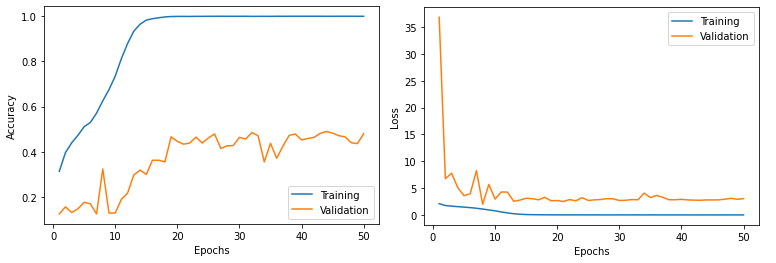
\includegraphics[scale=0.6]{images/2021-val-train.png}
\caption{CNN's Accuracy and Loss function of the training and validation set.}
\label{fig:Acc_Loss_2021}
\end{figure}


\begin{figure}[ht]
\centering
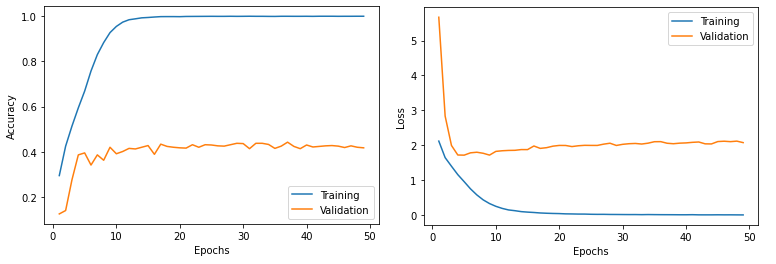
\includegraphics[scale=0.6]{images/tuned-val-train.png}
\caption{Tuned CNN's Accuracy and Loss function of the training and validation set.}
\label{fig:Acc_Loss_tuned}
\end{figure}

\begin{figure}
  \begin{subfigure}[c]{0.475\textwidth}
    \centering
    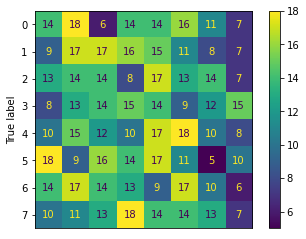
\includegraphics[width=\textwidth]{images/2021-confusion_matrix.png}
    \caption{Simple CNN}
    \label{fig:cf_2021}
  \end{subfigure}
  \hfill
  \begin{subfigure}[c]{0.475\textwidth}
      \centering
      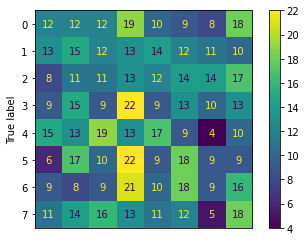
\includegraphics[width=\textwidth]{images/tuned-confusion_matrix.png}
      \caption{Tuned CNN}
      \label{fig:cf_tuned}
  \end{subfigure}
  \caption{CNN's confusion matrix.}
\end{figure}

\begin{figure}[ht]
\centering
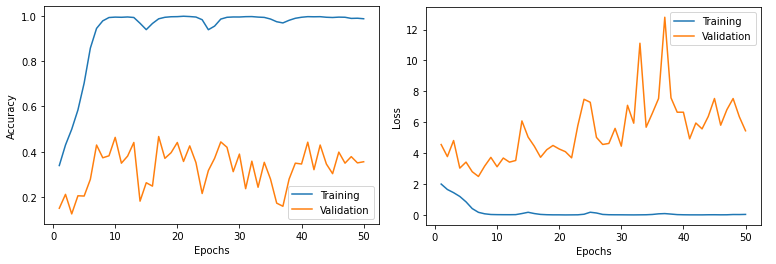
\includegraphics[scale=0.6]{images/aug-2021-val-train.png}
\caption{CNN's Accuracy and Loss function of the training and validation set with data augmentation.}
\label{fig:Acc_Loss_2021_aug}
\end{figure}

\begin{figure}[ht]
\centering
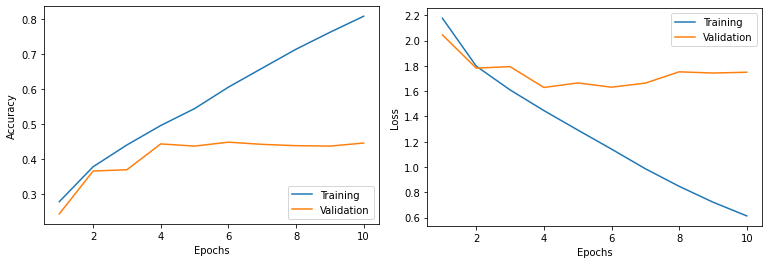
\includegraphics[scale=0.6]{images/aug-tuned-val-train.png}
\caption{Tuned CNN's Accuracy and Loss function of the training and validation set with data augmentation.}
\label{fig:Acc_Loss_tuned_aug}
\end{figure}

\begin{figure}
  \begin{subfigure}[c]{0.475\textwidth}
      \centering
      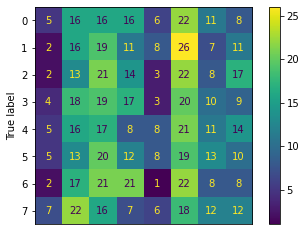
\includegraphics[width=\textwidth]{images/aug-2021-confusion_matrix.png}
      \caption{Simple CNN}
      \label{fig:cf_2021_aug}
  \end{subfigure}
  \hfill
  \begin{subfigure}[c]{0.475\textwidth}
      \centering
      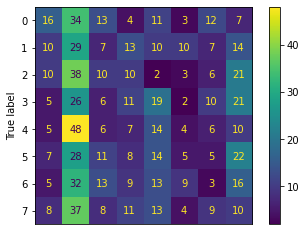
\includegraphics[width=\textwidth]{images/aug-tuned-confusion_matrix.png}
      \caption{Tuned CNN}
      \label{fig:cf_tuned_aug}
  \end{subfigure}
  \caption{CNN's confusion matrix with data augmentation.}
\end{figure}

\begin{table}[ht]
\centering
\resizebox{\textwidth}{!}{%
\begin{tabular}{|c|c|c|c|c|ccc|}
\hline
\multirow{2}{*}{Cut Level} & \multirow{2}{*}{Size} & \multirow{2}{*}{Size after PCA} & \multirow{2}{*}{PCA value} & \multirow{2}{*}{Model} & \multicolumn{3}{c|}{Accuracy}                                                           \\ \cline{6-8} 
                            &                       &                                 &                            &                        & \multicolumn{1}{c|}{svm linear}    & \multicolumn{1}{c|}{svm rbf}       & mlp           \\ \hline
Fc2                        & 4096                  & 1480                            & 0.99                       & VGG16                  & \multicolumn{1}{c|}{0.4440/0.4003} & \multicolumn{1}{c|}{0.5168/0.4454} & 0.4795/0.4191 \\ \hline
Fc2                        & 4096                  & 429                             & 0.95                       & VGG16                  & \multicolumn{1}{c|}{0.4965/0.4530} & \multicolumn{1}{c|}{0.5206/0.4542} & 0.4890/0.4361 \\ \hline
Fc2                        & 4096                  & 153                             & 0.9                        & VGG16                  & \multicolumn{1}{c|}{0.5099/0.4586} & \multicolumn{1}{c|}{0.5195/0.4617} & 0.4920/0.4398 \\ \hline
\end{tabular}%
}
\caption{...}
\label{tab:my-table}
\end{table}



\begin{table}[ht]
\centering
\resizebox{\textwidth}{!}{%
\begin{tabular}{|c|c|c|c|ccc|}
\hline
\multirow{2}{*}{Cut Level} & \multirow{2}{*}{Size} & \multirow{2}{*}{Size after PCA} & \multirow{2}{*}{Model} & \multicolumn{3}{c|}{Accuracy}                                                                     \\ \cline{5-7} 
                            &                       &                                 &                        & \multicolumn{1}{c|}{svm linear}    & \multicolumn{1}{c|}{svm rbf}                 & mlp           \\ \hline
Fc2                        & 4096                  & 153                             & VGG16                  & \multicolumn{1}{c|}{0.5099/0.4586} & \multicolumn{1}{c|}{0.5195/0.4617}           & 0.4920/0.4398 \\ \hline
Fc1                        & 4096                  & 311                             & VGG16                  & \multicolumn{1}{c|}{0.5157/0.4573} & \multicolumn{1}{c|}{0.5315/0.4837}           & 0.5076/0.4718 \\ \hline
block5\_pool               & 7x7x512               & 1174                            & VGG16                  & \multicolumn{1}{c|}{0.4316/0.4185} & \multicolumn{1}{c|}{\textbf{0.5317/ 0.4968}} & 0.4726/0.4429 \\ \hline
\end{tabular}%
}
\caption{...}
\label{tab:my-table}
\end{table}


\begin{table}[ht]
\centering
\resizebox{\textwidth}{!}{%
\begin{tabular}{|c|c|c|c|ccc|}
\hline
\multirow{2}{*}{Cut Level} & \multirow{2}{*}{Size} & \multirow{2}{*}{Size after PCA} & \multirow{2}{*}{Model} & \multicolumn{3}{c|}{Accuracy}                                                                    \\ \cline{5-7} 
                            &                       &                                 &                        & \multicolumn{1}{c|}{svm linear}    & \multicolumn{1}{c|}{svm rbf}                & mlp           \\ \hline
avg\_pool                  & 1000                  & 87                              & ResNet50               & \multicolumn{1}{c|}{0.5268/0.4649} & \multicolumn{1}{c|}{0.5381/0.4874}          & 0.5246/0.4592 \\ \hline
conv5\_block1\_2\_relu     & 7x7x512               & 1321                            & ResNet50               & \multicolumn{1}{c|}{0.4193/0.4104} & \multicolumn{1}{c|}{\textbf{0.5484/0.5012}} & 0.5221/0.4755 \\ \hline
\end{tabular}%
}
\caption{...}
\label{tab:my-table}
\end{table}

\begin{figure}
    \begin{subfigure}[c]{0.475\textwidth}
        \centering
        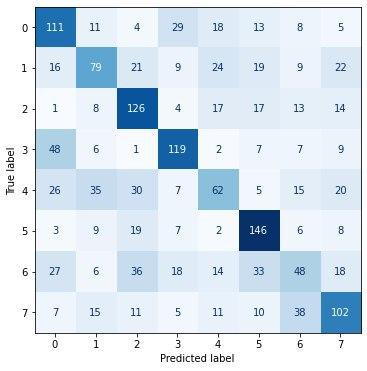
\includegraphics[width=\textwidth]{images/best_vgg16_svmrbf.jpg}
        \caption{aaaaa}
        \label{fig:best_vgg16_svmrbf_cm}
    \end{subfigure}
    \hfill
    \begin{subfigure}[c]{0.475\textwidth}
        \centering
        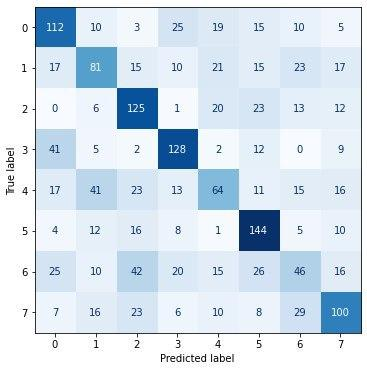
\includegraphics[width=\textwidth]{images/best_resnet50_svmrbf.jpg}
        \caption{bbbbb}
        \label{fig:best_resnet50_svmrbf_cm}
    \end{subfigure}
\end{figure}

\begin{table}[ht]
\centering
\resizebox{\textwidth}{!}{%
\begin{tabular}{|c|c|c|c|}
\hline
Model          & Test Time(CPU) & Test Time(GPU) & svm rbf   \\ \hline
vgg16\_best    & 60.6130 ms     & 3.2158 ms      & 4.4551 ms \\ \hline
resnet50\_best & 28.0918 ms     & 3.1582 ms      & 4.7911 ms \\ \hline
\end{tabular}%
}
\caption{...}
\label{tab:my-table}
\end{table}
